\begin{align}
\vec{D}=\frac{\vec{B}+\vec{C}}{2}
=\myvec{4\\ 0},
\\
	\vec{A}- \vec{B} =\myvec{1\\ -4},\,
	  \vec{A}- \vec{D} =\myvec{0\\ -6}
	  \\
	  \implies
  ar(ABD)=\frac{1}{2} \norm{\brak{\vec{A}-\vec{B}}  \times 
   \brak{\vec{A}- \vec{D}}} 
	       =3	
	       \\
	\vec{A}- \vec{C} =\myvec{-1\\ -8},\,
	  \vec{A}- \vec{D} =\myvec{0\\ -6}
	  \\
	  \implies
  ar(ACD)=\frac{1}{2} \norm{\brak{\vec{A}-\vec{C}}  \times 
   \brak{\vec{A}- \vec{D}}} 
   \\
	= 3 =
ar(ABD)
\end{align}
See  
\figref{fig:10/7/3/5/}.
\begin{figure}[H]
\centering
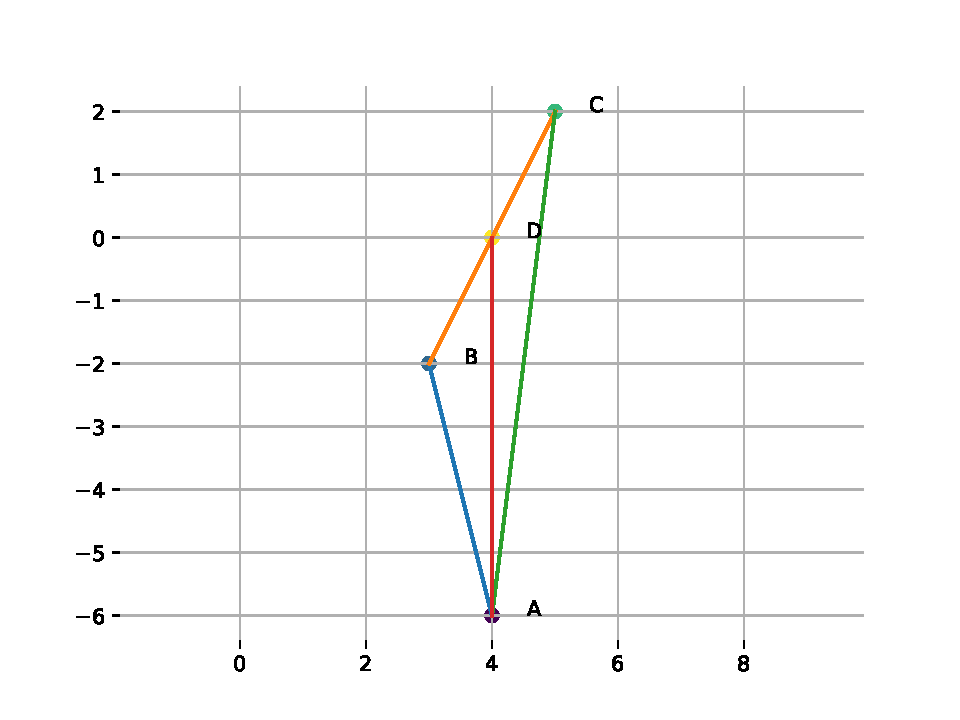
\includegraphics[width=0.75\columnwidth]{chapters/10/7/3/5/figs/fig.pdf}
\caption{}
\label{fig:10/7/3/5/}
\end{figure} 
